\documentclass[conference]{IEEEtran}
\IEEEoverridecommandlockouts

\usepackage{cite}
\usepackage{amsmath,amssymb,amsfonts}
\usepackage{algorithmic}
\usepackage{algorithm}
\usepackage{graphicx}
\usepackage{textcomp}
\usepackage{xcolor}
\usepackage{booktabs}
\usepackage{float}
\usepackage{multirow}
\usepackage{url}

\def\BibTeX{{\rm B\kern-.05em{\sc i\kern-.025em b}\kern-.08em
    T\kern-.1667em\lower.7ex\hbox{E}\kern-.125emX}}

\begin{document}

\title{NetGuard: Wire-to-Component Joining for\\Scanned Circuit Diagram Digitization}

\author{%
\IEEEauthorblockN{Bosco Chanam}
\IEEEauthorblockA{Symbiosis Centre for Applied AI\\
Symbiosis Institute of Technology\\
Pune, India\\
bosco.chanam.btech2021@sitpune.edu.in}
\and
\IEEEauthorblockN{Chris Dcosta}
\IEEEauthorblockA{Symbiosis Centre for Applied AI\\
Symbiosis Institute of Technology\\
Pune, India\\
chrisdcosta777@gmail.com}
\and
\IEEEauthorblockN{Pranavesh Kumar Talupuri}
\IEEEauthorblockA{Department of Computer Science\\
University of Southern California\\
Los Angeles, USA\\
talupuri@usc.edu}
}

\maketitle

\begin{abstract}
Scanned circuit digitization pipelines can often recover component instances and wire fragments, yet they still fail at the \emph{joining} step: deciding which detected wire endpoints connect to which component pins and neighboring wire segments. This paper focuses on that bottleneck. We formulate joining as a typed endpoint graph over wire endpoints and component pins, then add guarded floating-pin completion to recover plausible missing joins without introducing widespread false shorts. The full method, \emph{NetGuard}, improves the detected-scan structural error score from 0.3679 to 0.2710 relative to the \mbox{(1)+(2)} endpoint-graph-plus-rescue variant while maintaining 99.4\% wire usage, and reaches 0.9416 join F1 at the highest synthetic error severity. Because the scanned corpus lacks net-level ground truth, we separate real-image structural verification from synthetic net-level robustness tests and do not claim full real-world netlist correctness.
\end{abstract}

\begin{IEEEkeywords}
circuit digitization, document understanding, wire joining, graph-based connectivity, SPICE netlist extraction, analog circuit schematics
\end{IEEEkeywords}

\begin{figure*}[t]
\centering
\includegraphics[width=\textwidth]{figures/tikz/pipeline_overview_tikz.pdf}
\caption{Pipeline overview. The detector-support stages provide component priors and wire fragments as supporting context, while the highlighted join-recovery stages form the main contribution of the paper. NetGuard operates after fragment detection, converting the typed endpoint graph into recovered electrical nets and a SPICE-ready netlist.}
\label{fig:pipeline}
\end{figure*}

\begin{figure*}[t]
\centering
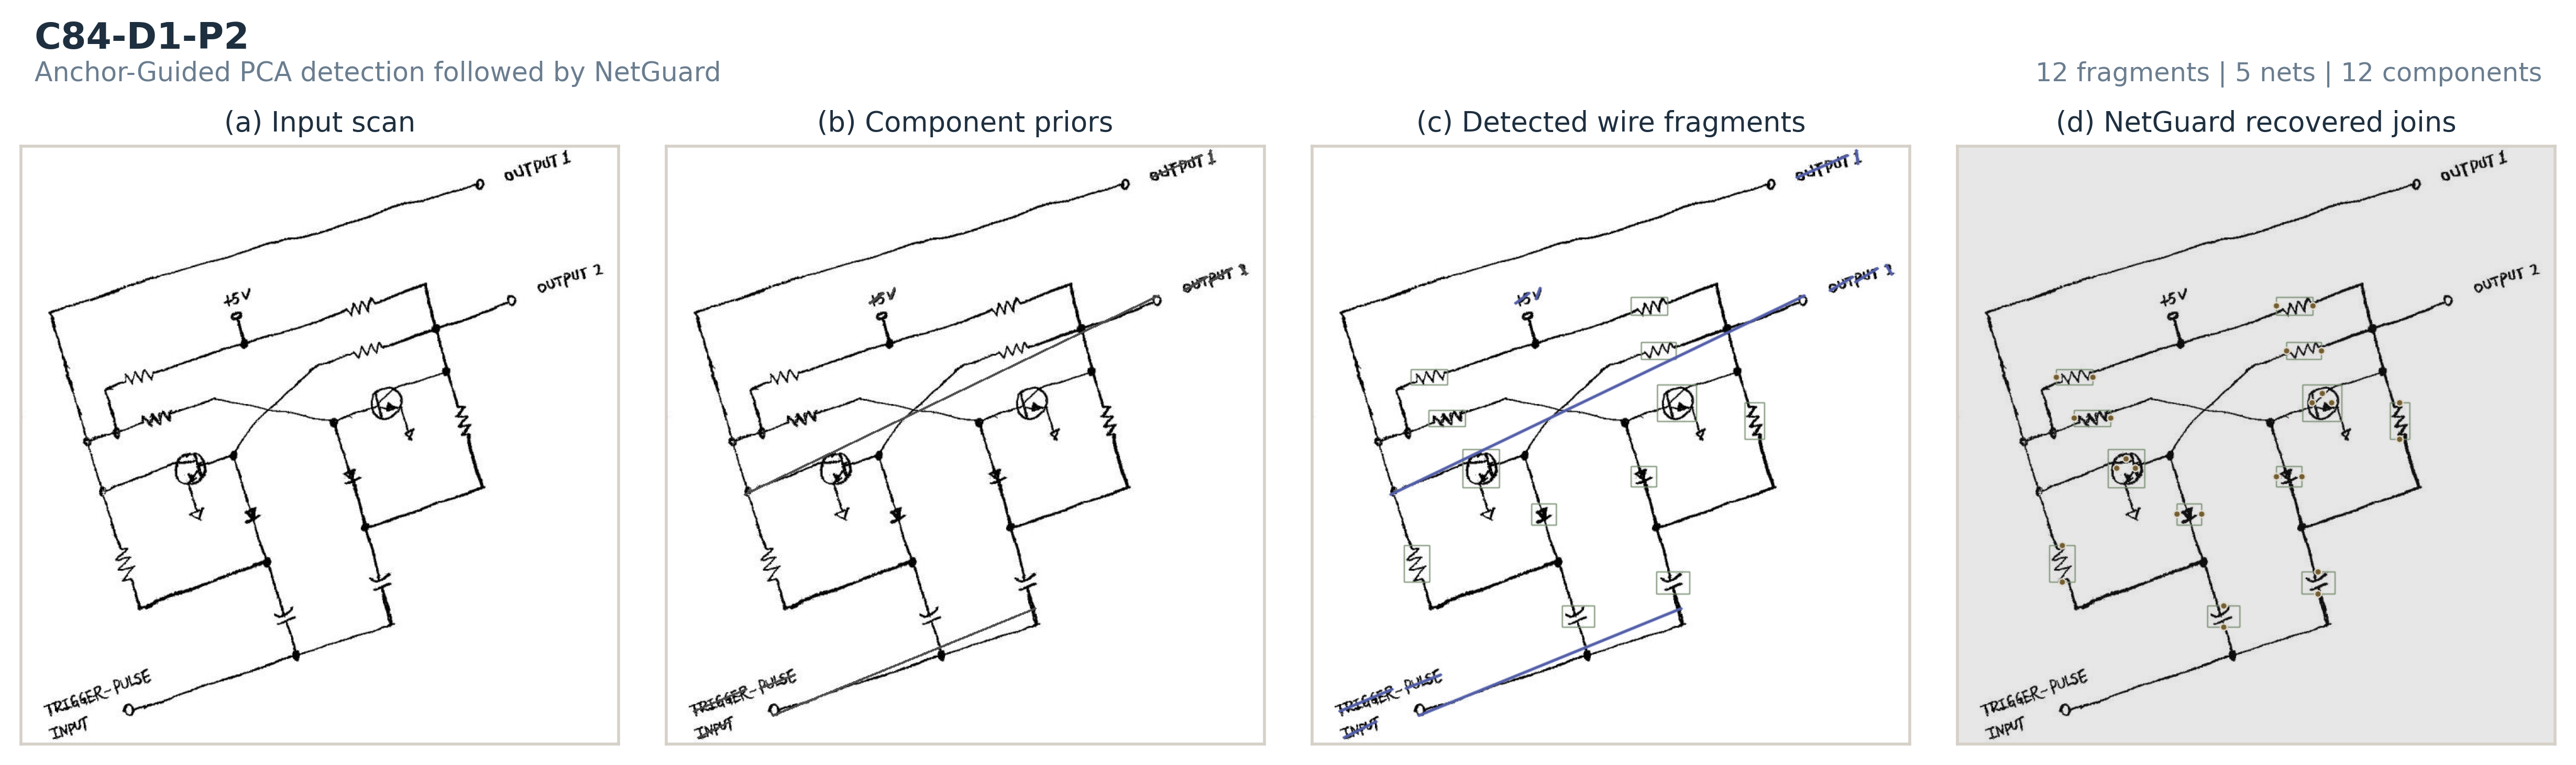
\includegraphics[width=0.86\textwidth]{figures/pipeline_examples/C84-D1-P2-jpg.png}
\caption{End-to-end behavior on a representative real scanned schematic. The figure keeps four readable stages: (a) input scan, (b) component priors and occlusion, (c) detected wire fragments, and (d) NetGuard recovered joins. This case contains 12 detected wire fragments, 5 recovered nets, and 12 nontrivial components, illustrating that the main ambiguity lies in converting plausible fragments into stable electrical joins.}
\label{fig:pipeline_examples}
\end{figure*}

\section{Introduction}

Analog circuit schematics encode component identity, electrical connectivity, and design intent in a visual form meant for human readers. Converting scanned schematics into machine-readable SPICE netlists would enable simulation, archival search, and downstream circuit analysis, but robust end-to-end digitization remains difficult. In our pipeline, the dominant failure mode is not component recognition or even raw wire extraction; it is the \emph{joining} step that decides which detected wire fragments belong to the same electrical net.

That joining problem is brittle for three geometric reasons. First, endpoint locations inferred from thresholded scans are noisy and may shift by tens of pixels across drawing styles. Second, components occupy regions that partially occlude the wire segments that should attach to their pins. Third, corners, T-junctions, near-misses, and dense local layouts create cases where a simple ``attach everything within a radius'' rule incorrectly shorts unrelated terminals.

Direct vision-language-model netlist transcription is attractive as a motivating alternative, but in our experiments it still under-specifies terminal connectivity and yields free-form text rather than a constrained electrical representation. We therefore keep the circuit-to-netlist path explicit and geometric.

The contribution hierarchy in this paper is deliberately narrow. Wire detection is supporting context, not the main claim. The paper's main contribution is the join-recovery stage, which we present as \emph{NetGuard}. More specifically, we 1) formalize joining as a typed endpoint graph over wire endpoints and component pins, 2) add guarded floating-pin completion that recovers plausible missing joins while limiting false shorts, and 3) evaluate the resulting joiner with three separate evidence layers: real detected-scan structural verification, synthetic perturbation robustness, and downstream simulation checks. Because the scanned corpus lacks net-level ground truth, we keep those evidence layers separate and do not overclaim full real-world netlist correctness.

\section{Related Work}

Recent work on circuit-diagram digitization has made clear progress on task framing, datasets, and end-to-end prototypes. Thoma et al.~\cite{thoma2021dataset} introduced a public handwritten-circuit dataset that helped move the problem from bespoke examples toward reproducible evaluation. Kelly and Cole~\cite{kelly2024digitizing} describe a configurable schematic-digitization pipeline that combines symbol interpretation, OCR, and graph construction, while Hemker et al.~\cite{hemker2024schematics} present a deep-learning-based route from schematics to netlists. Rachala and Panicker~\cite{rachala2022handdrawn} focus on hand-drawn circuit recognition using object detection and node recognition. Together, these papers show that end-to-end circuit parsing is feasible, but they also suggest that connectivity recovery remains fragile once wires are noisy, fragmented, or only partially visible.

That observation is consistent with the broader engineering-diagram literature. Large gains have been reported for symbol detection and classification in technical drawings~\cite{elyan2020symbols,lee2020engineering,yang2024singleline}, and Moreno-Garcia et al.~\cite{moreno2024review} review how deep learning has improved diagram digitization across multiple engineering domains. However, these systems still require domain-aware reasoning about lines, ports, and structural relationships after the detector stage. Even in closely related handwritten-diagram settings, such as Arrow R-CNN for hand-drawn diagrams~\cite{schaefer2021arrow}, the main challenge shifts from recognizing local shapes to recovering the relations between them.

The preprocessing choices in our pipeline also have a substantial literature behind them. Adaptive thresholding methods such as Otsu, Niblack, and Sauvola remain standard references when thin strokes must be separated from uneven backgrounds~\cite{otsu1979,niblack1986,sauvola2000}, and later document-image work refined those ideas for degraded pages and locally varying contrast~\cite{gatos2006,shafait2008,su2013}. Likewise, thinning, skeletonization, and line-recovery methods have long emphasized topology preservation over purely pixelwise segmentation quality~\cite{zhang1984thinning,lam1992thinning,duda1972hough,gioi2010lsd}. Those classical results remain relevant here because a joiner only has a chance to succeed if the upstream representation preserves the right sparse geometry.

What is still underdeveloped in the literature is a dedicated treatment of joining under detector error. Prior circuit papers usually treat connectivity as a downstream consequence of detection, often through Hough-style rules, nearest-node heuristics, or fixed-radius attachment~\cite{rachala2022handdrawn,hemker2024schematics}, and they rarely separate detector quality from join quality with distinct metrics. Vision-language-model approaches can help with high-level interpretation~\cite{kulkarni2025enhancing}, but they do not by themselves provide a verifiable electrical join structure. Our contribution is therefore narrower than a full digitization system: we isolate the wire-to-component joining stage, model it geometrically, and study how to recover plausible missing joins without paying for that recovery with a surge in false shorts.

\section{Method}

The end-to-end pipeline is summarized in Fig.~\ref{fig:pipeline}. Component priors come from oriented bounding-box detection. For the supporting wire stage, we use a component-guided classical detector that occludes component polygons with local median fill, thresholds the component-union crop with Sauvola binarization, applies light morphological closing, extracts connected components, estimates endpoints with PCA, and suppresses duplicate segments through overlap-aware filtering. The current traceable broad-benchmark artifact for that detector is the \emph{Anchor-Guided PCA Detector}, which provides the wire fragments consumed by every joining experiment reported here. We include that detector only as upstream context; the contribution of this paper begins after wire fragments and component pins have been proposed.

We use the following shorthand throughout: \textbf{(1)} typed endpoint graph, \textbf{(2)} dangling-end rescue, \textbf{(3)} floating-pin completion, and \textbf{(4)} degree budget plus self-loop guard. NetGuard denotes the full \textbf{(1)+(2)+(3)+(4)} method.

Joining begins with \textbf{(1)} typed endpoint graph construction. We form a graph from wire segments $\mathcal{W} = \{w_1, \ldots, w_m\}$ and component pins $\mathcal{P} = \{p_1, \ldots, p_n\}$, with nodes $V = \mathrm{eps}(\mathcal{W}) \cup \mathcal{P}$. For every wire $w_i$ with endpoints $(a_i, b_i)$, we add a zero-cost wire-body edge $(a_i, b_i)$ so both endpoints of an extracted segment remain electrically tied. Endpoint-endpoint edges connect nearby fragment ends when $\lVert e_i - e_j \rVert \leq \tau_{\mathrm{join}}$. Endpoint-pin edges connect an endpoint $e$ to a candidate pin $p$ when $\lVert e - p \rVert \leq \tau_{\mathrm{pin}}$, with weight $\lVert e - p \rVert (1 - \alpha \cos \theta)$ so the preferred attachment aligns with the local wire direction. Endpoint-wire-body edges connect a terminal endpoint to a passing wire body when the point-to-segment distance is below $\tau_t$, capturing T-junction behavior. For comparison, the \emph{Legacy Radius-Based Joiner} attaches each endpoint to every pin within a fixed 30\,px radius rather than using this typed graph.

All geometric tolerances are scale-relative, $\tau = k s$, where $s$ is the median component diagonal. Endpoint-pin hypotheses use a component-first assignment rule: an endpoint is first assigned to the nearest component by oriented-box distance, then mapped to a pin on that component by local geometry. This step is important when a detector places an endpoint inside a component box but not directly on the pin location.

\textbf{(2)} dangling-end rescue extends a subset of dangling wire endpoints directionally before graph construction or candidate generation. This stage is meant to recover short gaps caused by endpoint truncation. The \textbf{(1)+(2)} variant is the current endpoint-graph-plus-rescue baseline used throughout the results.

\begin{figure*}[t]
\centering
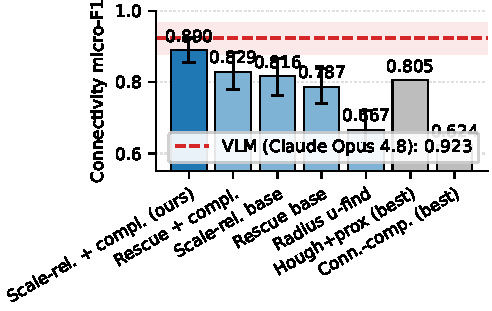
\includegraphics[width=\textwidth]{figures/real_join_comparison.png}
\caption{Real scanned-circuit join comparison on case \texttt{C84\_D1\_P2}. Panel (a) shows that the Legacy Radius-Based Joiner over-merges nearby attachments into one oversized net. Panel (b) shows the same crop under NetGuard, with the zoomed inset highlighting the preserved separation. The figure supports the paper's central real-image claim: join quality changes materially even when the upstream wire detector is unchanged.}
\label{fig:real_join}
\end{figure*}

The endpoint graph is converted to nets by connected components over $G$, projected onto pins. This base join is intentionally conservative, so it may leave some terminals \emph{floating}: a pin lands in a net that contains only pins from its own component after inert classes such as ground, terminal, and text are excluded. \textbf{(3)} floating-pin completion starts from those terminals and generates candidate completion edges to plausible pins on other components. \textbf{(4)} degree budget plus self-loop guard limits how many completion edges can target a pin and rejects same-component completions or merges that would create component self-loops. NetGuard is the full \textbf{(1)+(2)+(3)+(4)} combination.

\begin{algorithm}[t]
\caption{NetGuard: Guarded Floating-Pin Completion}
\label{alg:degree_budget}
\begin{algorithmic}[1]
\STATE Run the \textbf{(1)+(2)} endpoint-graph join and compute provisional nets.
\STATE Mark a pin $p$ as floating if its net contains only pins from $p$'s own component.
\FOR{each floating pin $p$}
\STATE Generate candidate edges $(p, q)$ to pins on other components within reach $r = 2.5s$.
\STATE Weight each candidate by Euclidean distance between $p$ and $q$.
\ENDFOR
\STATE Apply \textbf{(4)} degree budgets and self-loop guards during completion selection.
\STATE Solve a min-cost b-matching problem with at most one assignment per floating pin.
\STATE Allow each target pin up to three slots and include an opt-out assignment.
\FOR{each selected candidate edge $(p, q)$}
\IF{$p$ and $q$ belong to the same component}
\STATE Reject the edge.
\ELSIF{merging the two nets would create a component self-loop}
\STATE Reject the edge.
\ELSE
\STATE Merge the two nets with an inferred completion edge.
\ENDIF
\ENDFOR
\STATE Return the completed pin-to-net mapping.
\end{algorithmic}
\end{algorithm}

The completion stage is shown conceptually in Fig.~\ref{fig:completion}. NetGuard is the full \textbf{(1)+(2)+(3)+(4)} method. Its implementation details are compact but important for reproducibility. The characteristic scale $s$ is the median component diagonal. The \textbf{(2)} rescue stage applies a single 12\,px end extension before graph construction. Variant \textbf{(3)} uses candidate reach $2.5s$, and the full NetGuard method adds \textbf{(4)} degree budgets together with a self-loop guard that rejects any candidate merge between nets that already share a component. The assignment routine is the Hungarian solver from \texttt{scipy.optimize.linear\_sum\_assignment}~\cite{kuhn1955}. Completion edges are wireless: they represent inferred schematic joins rather than newly hallucinated wire geometry. We also compare \textbf{(1)} endpoint graph only, which shares the same graph view but omits both rescue and floating-pin completion. For the detected-scan verification reported later, we summarize join quality with a \emph{structural error score} defined as
\[
\text{structural error score} = \text{composite} + 0.5 \cdot \frac{\text{unused wires}}{\max(1,\text{all wires})},
\]
where the composite term counts self-loops, floating components, and giant nets per component. Lower values are better because they indicate fewer over-merge and under-connection failures on detected scans.

\begin{figure*}[t]
\centering
\includegraphics[width=\textwidth]{figures/tikz/netguard_concept_tikz.pdf}
\caption{NetGuard concept. The figure visualizes the four stages reused throughout the paper: (1) typed endpoint graph, (2) dangling-end rescue, (3) floating-pin candidate generation, and (4) guarded completion with degree budgets and self-loop rejection. Dashed edges denote candidate completions, the thick solid edge denotes the accepted completion, and the rejected edge illustrates the structural guard against false shorts.}
\label{fig:completion}
\end{figure*}

\subsection{Synthetic Evaluation Framework}

The real scanned corpus gives wire-level and component-level labels, but it does not provide net-level ground truth. That prevents direct scoring of correct electrical joining on real images and motivates a separate synthetic benchmark. We therefore use the synthetic benchmark as a robustness proxy rather than a replacement for the real-image evaluation.

We author 15 synthetic circuits spanning 3--6 components and 2--6 nets, including dividers, RC/RL chains, diode loops, bridge structures, and cyclic topologies. Each circuit has a known ground-truth netlist and a corresponding SPICE deck. Error injection is designed to approximate the detector-side failures that the joiner actually sees. Across four nonzero severity levels on top of the clean control, we perturb endpoints with Gaussian jitter from 3\,px to 14\,px, shorten wires by 4--22\,px to model endpoints that stop short of a pin, drop whole wires with probability up to 0.20, snap some endpoints to the wrong nearby pin with probability up to 0.10, and displace one endpoint by as much as 80\,px under the most severe setting. The primary synthetic metric is join F1, measured over component pairs that should or should not share a net. We also report simulation accuracy (\texttt{sim\_ok}), the percentage of random seeds whose recovered SPICE deck preserves every authored source current within tolerance relative to the clean oracle. Join precision falls when false shorts appear, while join recall falls when fragmentation leaves intended component pairs disconnected.

\begin{table*}[t]
\caption{Evidence layers used in the paper.}
\label{tab:protocol}
\begin{center}
\scriptsize
\begin{tabular}{p{3.05cm}p{3.0cm}p{2.55cm}p{5.7cm}}
\toprule
\textbf{Evidence Layer} & \textbf{Evaluation Unit} & \textbf{Main Metrics} & \textbf{Purpose} \\
\midrule
Supporting detector context & Detected wire fragments on broad and stress subsets & F1, precision, recall & Fix the upstream wire evidence consumed by every join experiment and show that the joiner is not being credited for detector quality \\
Real scanned structural verification & Pin-to-net structure on detected scans & Structural error, wires used, floating components, self-loops & Measure whether a joiner over-merges attachments or leaves many fragments unused on real scans \\
Synthetic net-level robustness & Component-pair connectivity under controlled perturbations & Precision, recall, F1 & Measure robustness to dropped, shifted, and truncated endpoints when exact net-level ground truth is available \\
Downstream simulation sanity check & Recovered SPICE deck on representative L4 synthetic cases & \texttt{sim\_ok} & Check whether fragmentation failures preserve or break simple operating-point behavior on representative circuits \\
\bottomrule
\end{tabular}
\normalsize
\end{center}
\end{table*}

\section{Results}

The results are organized around the three evidence layers promised in the introduction. We first define those layers, then summarize the main join results, and finally unpack real scanned behavior, synthetic robustness, and the remaining simulation and detector context.

\begin{table*}[t]
\caption{Join results under a fixed detector input. All join experiments use the same wire fragments from the Anchor-Guided PCA Detector, so detector quality is held fixed across rows. Lower structural error is better.}
\label{tab:main_summary}
\begin{center}
\scriptsize
\resizebox{\textwidth}{!}{%
\begin{tabular}{lcccccccc}
\toprule
\textbf{Method / Variant} & \textbf{Structural Error $\downarrow$} & \textbf{Wires Used $\uparrow$} & \textbf{Floating $\downarrow$} & \textbf{Self-Loops $\downarrow$} & \textbf{L4 Precision $\uparrow$} & \textbf{L4 Recall $\uparrow$} & \textbf{L4 F1 $\uparrow$} & \textbf{Mean sim\_ok $\uparrow$} \\
\midrule
Legacy Radius Joiner & --- & --- & --- & --- & 0.6444 & 0.2757 & 0.3635 & --- \\
\textbf{(1) Endpoint graph} & 0.3610 & \textbf{99.5\%} & 1726 & \textbf{62} & \textbf{0.9843} & 0.7933 & 0.8497 & --- \\
\textbf{(1)+(2) Endpoint graph + rescue} & 0.3679 & 99.4\% & 1607 & 213 & 0.9743 & 0.8619 & 0.8985 & --- \\
\textbf{NetGuard} & \textbf{0.2710} & 99.4\% & \textbf{1084} & 213 & 0.9716 & \textbf{0.9279} & \textbf{0.9416} & 33.4\% \\
\bottomrule
\end{tabular}
}
\normalsize
\end{center}
\end{table*}
% TODO: Add an explicit (1)+(2)+(3) completion-without-guard row once a stable
% registry entry or archived benchmark artifact exists for the unguarded variant.

\begin{table*}[t]
\caption{Detected-scan structural error decomposition for the graph-based variants. These counts explain why NetGuard lowers the real-image structural score: floating components drop sharply, while giant-net growth remains modest.}
\label{tab:struct_decomp}
\begin{center}
\scriptsize
\begin{tabular}{lrrrr}
\toprule
\textbf{Variant} & \textbf{Floating $\downarrow$} & \textbf{Self-Loops $\downarrow$} & \textbf{Giant Nets $\downarrow$} & \textbf{Wires Used $\uparrow$} \\
\midrule
\textbf{(1) Endpoint graph} & 1726 & \textbf{62} & \textbf{86} & \textbf{99.5\%} \\
\textbf{(1)+(2) Endpoint graph + rescue} & 1607 & 213 & 102 & 99.4\% \\
\textbf{NetGuard} & \textbf{1084} & 213 & 109 & 99.4\% \\
\bottomrule
\end{tabular}
\normalsize
\end{center}
\end{table*}

Table~\ref{tab:protocol} defines the evidence layers compactly, and the main caveat is important: the real scanned corpus does not provide net-level ground truth. Real-image numbers therefore use structural verification rather than literal net correctness, the synthetic benchmark provides controlled net-level robustness evidence, and the simulation checks are downstream sanity checks rather than full SPICE-equivalence proofs.

Table~\ref{tab:main_summary} then summarizes the paper's central quantitative claim. NetGuard gives the best trade-off between real scanned structure and synthetic robustness under the current evidence. On detected scans, it lowers the structural error score from 0.3679 to 0.2710 relative to the \mbox{(1)+(2)} endpoint-graph-plus-rescue variant while keeping wire usage unchanged at 99.4\%. Under the heaviest synthetic perturbation, it preserves substantially more recall than the lighter graph variants and clearly outperforms the Legacy Radius Joiner on both precision and F1.

The real scanned evidence is the most direct signal of practical behavior, but it remains a structural verification target rather than a net-level correctness score. Table~\ref{tab:struct_decomp} shows why the structural score moves. Relative to the \mbox{(1)+(2)} baseline, NetGuard removes 523 floating components on average while keeping wire usage unchanged and only modestly increasing the giant-net count from 102 to 109. The comparison with the \mbox{(1)} endpoint-graph variant is also informative: the plain graph keeps self-loops and giant nets low, but it leaves many more terminals unresolved. Figure~\ref{fig:real_join} shows the same effect visually on case \texttt{C84\_D1\_P2}. The highlighted inset in the legacy panel shows a local over-merge region where nearby attachments collapse into an oversized net. The corresponding inset in the NetGuard panel shows the same area after guarded completion, where the intended separation is preserved.

\begin{figure*}[t]
\centering
\includegraphics[width=\textwidth]{figures/join_robustness_breakdown.pdf}
\caption{Synthetic robustness decomposition. Panels (a)--(c) show component-connectivity F1, precision, and recall across severity levels L0--L4 using the exact metric values reported in the paper. NetGuard is visually emphasized because it is the full proposed method, and the figure shows that its main gain over \mbox{(1)+(2)} comes from improved recall at high severity without a comparable loss in precision.}
\label{fig:join_robustness}
\end{figure*}

The synthetic benchmark answers a different question: how well does a joiner tolerate the kinds of endpoint noise, truncation, and missing fragments that a real detector produces? Figure~\ref{fig:join_robustness} makes the central pattern explicit. The graph-based variants all avoid the precision collapse of the Legacy Radius Joiner, but only NetGuard substantially restores recall at high severity. The resulting F1 gap at L4 is driven by fragmentation recovery rather than by a precision-for-recall trade: the full proposed method retains 0.9716 precision while improving recall to 0.9279, whereas the \mbox{(1)+(2)} endpoint-graph-plus-rescue variant reaches 0.9743 precision but only 0.8619 recall.

Because the synthetic benchmark is seed-driven, Appendix Table~\ref{tab:l4_uncertainty} reports the L4 mean and standard deviation across eight random seeds. The spread is largest in recall, which is consistent with fragmentation sensitivity under heavy perturbation. Even with that variability, NetGuard keeps the strongest mean L4 F1 among the compared joiners.

The simulation view supports the same interpretation. Errors mostly cause \emph{fragmentation}, not \emph{shorts}. Precision stays high even on the hardest synthetic cases, while simulation accuracy falls on cyclic or bridge-like circuits where a single missed connection can break a current path. The Wheatstone bridge and \texttt{ring6\_r} remain the clearest stress cases, and the mean L4 simulation accuracy across the representative suite is 33.4\%, which is consistent with a joiner that usually preserves local correctness but still fails when a single broken path disconnects a critical loop. Appendix Fig.~\ref{fig:ring6_failure} shows one such residual failure case for NetGuard on \texttt{ring6\_r}: the method preserves precision, but one missing link still fragments the cycle and depresses recall.

The detector evidence remains supporting context rather than the main novelty claim. The production detector is the Anchor-Guided PCA Detector, which supplies the fixed wire fragments for every join experiment. On the current traceable broad benchmark artifact it reaches F1~=~0.8605, precision~=~0.9261, and recall~=~0.8036 over 124 matched scans, with TP~=~3322, FP~=~221, and FN~=~812. On the curated 23-image stress subset it reaches F1~=~0.7492, while the specialized Hard-Case Recovery Detector reaches the strongest subset score at 0.8215. We therefore hold the Anchor-Guided PCA Detector fixed as the production wire source while recognizing that a specialized detector can outperform it on the hardest subset.

\section{Discussion}

The evidence supports a conservative but defensible claim. On real scanned schematics, the paper shows that join quality is not determined by detector F1 alone: two joiners can consume the same detected wire set and still produce materially different electrical structure. On synthetic perturbations, the paper shows that NetGuard recovers a failure mode that the lighter graph variants leave unresolved, namely floating terminals created by truncated or displaced endpoints. The main point is not that matching itself is novel; it is that guarded floating-pin completion can recover plausible edges while keeping hard structural limits in place.

The paper also has clear limitations. The real scanned benchmark offers structural verification and qualitative inspection, but it does not provide net-level ground truth, so it cannot certify that every recovered connection is electrically correct. The synthetic error model is therefore only a controlled proxy for detector noise, and it is not yet calibrated from a measured empirical error distribution. The method also depends on accurate component priors and inherits upstream errors from the detector, especially on faint traces, crowded local layouts, and ambiguous crossovers. In addition, the current structural error score is a surrogate for gross over-merge and under-connection behavior, not a literal electrical correctness metric. For that reason, the paper supports a narrow claim: under the current evidence, NetGuard is a stronger join-recovery stage. It does not yet prove full end-to-end netlist correctness on real scanned schematics.

\section{Future Scope}

The most important next step is a real scanned benchmark with net-level annotations so that join correctness can be measured directly rather than through structural surrogates. A second priority is to calibrate the synthetic perturbation model from observed detector failures instead of hand-specified ranges, which would tighten the link between the real and synthetic evidence layers. Beyond that, the framework should be extended to denser schematic styles and broader component families, and the downstream evaluation should move beyond operating-point preservation toward stronger graph-level and SPICE-level equivalence checks.

\section{Conclusion}

NetGuard improves the most fragile stage of scanned-circuit digitization: converting detected wire fragments into electrical nets. The contribution is strongest when interpreted narrowly. The method formalizes joining as a typed endpoint graph, adds guarded floating-pin completion on top of that graph, and improves both synthetic net-level robustness and real detected-scan structural verification without relying on a stronger detector. Within the current evidence stack, that is the central result of the paper.

\clearpage
\appendices
\section{Supplementary Tables}

\begin{table}[H]
\caption{Synthetic severity schedule used in the perturbation benchmark.}
\label{tab:severity}
\begin{center}
\scriptsize
\resizebox{\columnwidth}{!}{%
\begin{tabular}{lccc}
\toprule
\textbf{Level} & \textbf{Endpoint Jitter} & \textbf{Truncation} & \textbf{Extra Corruption} \\
\midrule
L1 & 3\,px & 4\,px & none \\
L2 & 6\,px & 8\,px & mild drop, pin snap \\
L3 & 10\,px & 16\,px & stronger drop, misassignment \\
L4 & 14\,px & 22\,px & 0.20 drop, 0.10 wrong pin, 80\,px shift \\
\bottomrule
\end{tabular}
}
\normalsize
\end{center}
\end{table}

\begin{table}[H]
\caption{Representative L4 NetGuard outcomes by circuit.}
\label{tab:per_circuit}
\begin{center}
\begin{tabular}{lrrrr}
\toprule
\textbf{Circuit} & \textbf{Comps} & \textbf{F1} & \textbf{Prec.} & \textbf{sim\_ok} \\
\midrule
parallel\_rr & 3 & 0.97 & 1.00 & 25\% \\
divider\_rr & 3 & 0.91 & 0.94 & 50\% \\
rl\_series & 3 & 0.91 & 1.00 & 62\% \\
diode\_r & 3 & 0.91 & 1.00 & 50\% \\
dense\_pair & 4 & 0.96 & 1.00 & 12\% \\
loop4\_r & 4 & 0.87 & 0.97 & 44\% \\
wheatstone & 6 & 0.76 & 0.85 & 12\% \\
ring6\_r & 6 & 0.79 & 0.97 & 12\% \\
\bottomrule
\end{tabular}
\end{center}
\end{table}

\begin{table}[H]
\caption{L4 synthetic uncertainty over eight random seeds and 15 circuits. Values are reported as mean $\pm$ standard deviation of the per-seed suite average.}
\label{tab:l4_uncertainty}
\begin{center}
\scriptsize
\resizebox{\columnwidth}{!}{%
\begin{tabular}{lccc}
\toprule
\textbf{Variant} & \textbf{Precision $\uparrow$} & \textbf{Recall $\uparrow$} & \textbf{F1 $\uparrow$} \\
\midrule
\textbf{(1) Endpoint graph} & $0.9843 \pm 0.0143$ & $0.7933 \pm 0.1851$ & $0.8497 \pm 0.1389$ \\
\textbf{(1)+(2) Endpoint graph + rescue} & $0.9743 \pm 0.0203$ & $0.8619 \pm 0.1109$ & $0.8985 \pm 0.0699$ \\
\textbf{NetGuard} & $0.9716 \pm 0.0210$ & $0.9279 \pm 0.0778$ & $0.9416 \pm 0.0455$ \\
\textbf{Legacy Radius Joiner} & $0.6444 \pm 0.4281$ & $0.2757 \pm 0.2301$ & $0.3635 \pm 0.2896$ \\
\bottomrule
\end{tabular}
}
\normalsize
\end{center}
\end{table}

\begin{figure*}[t]
\centering
\includegraphics[width=\textwidth]{figures/netguard_failure_ring6.png}
\caption{Residual synthetic failure case for NetGuard on \texttt{ring6\_r} at L4. The method preserves precision by avoiding a false short, but one missed link still fragments the six-component ring and limits recall. This is representative of the cyclic stress cases summarized in Table~\ref{tab:per_circuit}.}
\label{fig:ring6_failure}
\end{figure*}

\begin{table}[H]
\caption{Supporting detector context.}
\label{tab:wire_benchmark}
\begin{center}
\scriptsize
\resizebox{\columnwidth}{!}{%
\begin{tabular}{lccccc}
\toprule
\textbf{Detector} & \textbf{Broad F1 $\uparrow$} & \textbf{Prec. $\uparrow$} & \textbf{Rec. $\uparrow$} & \textbf{Stress F1 $\uparrow$} & \textbf{Suite F1 $\uparrow$} \\
\midrule
Anchor-Guided PCA Detector & 0.8605 & 0.9261 & 0.8036 & 0.7492 & 0.8049 \\
Hard-Case Recovery Detector & 0.7952 & --- & --- & 0.8215 & 0.8083 \\
Recall-Optimized Hybrid Detector & 0.8378 & --- & --- & 0.7595 & 0.7987 \\
Precision-Tuned Skeleton Detector & 0.7943 & --- & --- & 0.7830 & 0.7887 \\
\bottomrule
\end{tabular}
}
\normalsize
\end{center}
\end{table}

\clearpage
\begin{thebibliography}{00}
\bibitem{thoma2021dataset} F.~Thoma, J.~Bayer, Y.~Li, and A.~Dengel, ``A public ground truth dataset for handwritten circuit diagram images,'' in \textit{Proc. Int. Conf. Document Analysis and Recognition (ICDAR)}, 2021.
\bibitem{bayer2021cghd} J.~Bayer, ``CGHD-1152: Circuit graph hand-drawing dataset,'' Kaggle, 2021. [Online]. Available: \url{https://www.kaggle.com/datasets/johannesbayer/cghd1152}
\bibitem{kelly2024digitizing} C.~R.~Kelly and J.~M.~Cole, ``Digitizing images of electrical-circuit schematics,'' \textit{APL Mach. Learn.}, vol.~2, no.~1, p.~016109, 2024.
\bibitem{kulkarni2025enhancing} S.~Kulkarni \textit{et~al.}, ``Enhancing circuit diagram understanding via near sight correction using VLMs,'' in \textit{Proc. ICCV Workshops}, 2025.
\bibitem{rachala2022handdrawn} R.~R.~Rachala and M.~R.~Panicker, ``Hand-drawn electrical circuit recognition using object detection and node recognition,'' \textit{SN Comput. Sci.}, vol.~3, no.~3, p.~244, 2022.
\bibitem{hemker2024schematics} D.~Hemker, J.~Maalouly, H.~Mathis, R.~Klos, and E.~Ravanan, ``From schematics to netlists: electrical circuit analysis using deep-learning methods,'' \textit{Adv. Radio Sci.}, vol.~22, pp.~61--75, 2024.
\bibitem{elyan2020symbols} E.~Elyan, L.~Jamieson, and A.~Ali-Gombe, ``Deep learning for symbols detection and classification in engineering drawings,'' \textit{Neural Netw.}, vol.~129, pp.~91--102, 2020.
\bibitem{lee2020engineering} D.-Y.~Yun, S.-K.~Seo, U.~Zahid, and C.-J.~Lee, ``Deep neural network for automatic image recognition of engineering diagrams,'' \textit{Appl. Sci.}, vol.~10, no.~11, p.~4005, 2020.
\bibitem{yang2024singleline} L.~Yang, J.~Wang, J.~Zhang, H.~Li, K.~Wang, C.~Yang, and D.~Shi, ``Practical single-line diagram recognition based on digital image processing and deep vision models,'' \textit{Expert Syst. Appl.}, vol.~238, p.~122389, 2024.
\bibitem{moreno2024review} L.~Jamieson, C.~F.~Moreno-Garc{\'\i}a, and E.~Elyan, ``A review of deep learning methods for digitisation of complex documents and engineering diagrams,'' \textit{Artif. Intell. Rev.}, vol.~57, p.~136, 2024.
\bibitem{schaefer2021arrow} B.~Sch{\"a}fer, M.~Keuper, and H.~Stuckenschmidt, ``Arrow R-CNN for handwritten diagram recognition,'' \textit{Int. J. Document Anal. Recognit.}, vol.~24, no.~1--2, pp.~3--17, 2021.
\bibitem{otsu1979} N.~Otsu, ``A threshold selection method from gray-level histograms,'' \textit{IEEE Trans. Syst., Man, Cybern.}, vol.~9, no.~1, pp.~62--66, 1979.
\bibitem{niblack1986} W.~Niblack, \textit{An Introduction to Digital Image Processing}. Englewood Cliffs, NJ, USA: Prentice-Hall, 1986.
\bibitem{sauvola2000} J.~Sauvola and M.~Pietik{\"a}inen, ``Adaptive document image binarization,'' \textit{Pattern Recognit.}, vol.~33, no.~2, pp.~225--236, 2000.
\bibitem{gatos2006} B.~Gatos, I.~Pratikakis, and S.~J.~Perantonis, ``Adaptive degraded document image binarization,'' \textit{Pattern Recognit.}, vol.~39, no.~3, pp.~317--327, 2006.
\bibitem{shafait2008} F.~Shafait, D.~Keysers, and T.~M.~Breuel, ``Efficient implementation of local adaptive thresholding techniques using integral images,'' in \textit{Document Recognition and Retrieval XV}, vol.~6815, 2008, p.~681510.
\bibitem{su2013} B.~Su, S.~Lu, and C.~L.~Tan, ``Robust document image binarization technique for degraded document images,'' \textit{IEEE Trans. Image Process.}, vol.~22, no.~4, pp.~1408--1417, 2013.
\bibitem{zhang1984thinning} T.~Y.~Zhang and C.~Y.~Suen, ``A fast parallel algorithm for thinning digital patterns,'' \textit{Commun. ACM}, vol.~27, no.~3, pp.~236--239, 1984.
\bibitem{lam1992thinning} L.~Lam, S.-W.~Lee, and C.~Y.~Suen, ``Thinning methodologies: a comprehensive survey,'' \textit{IEEE Trans. Pattern Anal. Mach. Intell.}, vol.~14, no.~9, pp.~869--885, 1992.
\bibitem{duda1972hough} R.~O.~Duda and P.~E.~Hart, ``Use of the Hough transformation to detect lines and curves in pictures,'' \textit{Commun. ACM}, vol.~15, no.~1, pp.~11--15, 1972.
\bibitem{gioi2010lsd} R.~Grompone von Gioi, J.~Jakubowicz, J.-M.~Morel, and G.~Randall, ``LSD: a fast line segment detector with a false detection control,'' \textit{IEEE Trans. Pattern Anal. Mach. Intell.}, vol.~32, no.~4, pp.~722--732, 2010.
\bibitem{kuhn1955} H.~W.~Kuhn, ``The Hungarian method for the assignment problem,'' \textit{Naval Res. Logist. Quart.}, vol.~2, no.~1--2, pp.~83--97, 1955.
\end{thebibliography}

\end{document}
